\documentclass{article}
\usepackage{qilin}
\tikzstyle{process} = [rectangle, rounded corners, minimum width=1.5cm, minimum height=0.5cm,align=center, draw=black, fill=gray!30, auto]
\title{PHY294: Practice Problems \\ \textbf{Problem Set 1 Solutions}}
\author{QiLin Xue}
\date{Winter 2022}
\usepackage{mathrsfs}
\usetikzlibrary{arrows}
\begin{document}

\maketitle
\begin{enumerate}[label=(8.\arabic*)]
    \setcounter{enumi}{3}

    \item The Schrödinger equation is (in 3D)
    \begin{equation*}
        E \psi = -\frac{\hbar^2}{2m} \left(\frac{\partial^2}{\partial x^2} + \frac{\partial^2}{\partial y^2} + \frac{\partial^2}{\partial z^2}\right) \psi
    \end{equation*}
    Substituting $\psi = e^{i\bm{k}\cdot\bm{r}}=e^{i(k_xx+k_yy+k_zz)}=e^{ik_xx}e^{ik_yy}e^{ik_zz},$ we get 
    \begin{equation*}
        Ee^{ik_xx}e^{ik_yy}e^{ik_zz} = -\frac{\hbar^2}{2m}\left(-k_x^2-k_y^2-k_z^2\right)e^{ik_xx}e^{ik_yy}e^{ik_zz}
    \end{equation*}
    or
    \begin{equation*}
        E = \frac{\hbar^2}{2m} \bm{k}^2,
    \end{equation*}
    as desired. We can interpret $\bm{k}$ as the \emf{wave vector}.
    \item \begin{enumerate}
        \item The quantity $\frac{\partial h}{\partial x}$ represents the slope in the eastwards direction.
        \item The quantity $\frac{\partial h}{\partial y}$ represents the slope in the northwards direction.
        \item The hiker remains at the same elevation though he will be walking on a slanted path.
    \end{enumerate}
    \setcounter{enumi}{8}
    \item Consider the wavefunction to be in the form of $\psi(x,y) = \phi(x)\phi(y).$ Then applying the 2D Schrodinger equation, we have:
    \begin{equation*}
        E\phi(x)\phi(y) = -\frac{\hbar^2}{2m}\left(\phi(y)\frac{\partial^2}{\partial x^2}\phi(x) + \phi(x)\frac{\partial^2}{\partial y^2}\phi(y)\right).
    \end{equation*}
    Rearranging such that everything with an $x$ dependence is on the left side, we get 
    \begin{equation*}
        \frac{1}{\phi(x)}\frac{\partial^2 \phi(x)}{\partial x^2} = -\left(\underbrace{\frac{2ME}{\hbar^2}+\frac{1}{\phi(y)}\frac{\partial^2 \phi(y)}{\partial y^2}}_{k_x^2}\right)
    \end{equation*}
    The right-hand side is independent of $x$, so we can solve this differential equation normally and end up with
    \begin{equation*}
        \phi(x) = A\sin(k_xx) = A\sin\left(\frac{n_x\pi}{a}\right),
    \end{equation*}
    which comes from the boundary conditions, similar to how we found the solution to the 1-D box. Similarly, we can do the same thing in the $y$ direction to get 
    \begin{equation*}
        \phi(y) = B\sin\left(\frac{n_y\pi}{b}\right).
    \end{equation*}
    Making the substitutions $\frac{1}{\phi(x)}\frac{\partial^2 \phi(x)}{\partial x^2} = -k_x^2$ and $\frac{1}{\phi(y)}\frac{\partial^2 \phi(y)}{\partial y^2} = -k_y^2$, we get
    \begin{equation*}
        k_x^2+k_y^2 = \frac{2ME}{\hbar^2},
    \end{equation*}
    and using the relationship between $k$ and $n$, we get the desired form.

    \emf{Remarks:} This $k$ wave vector is the same as the one in question 8.4. Thus, it can be solved directly using the earlier relationship without using separation of variables, or even solving it!
    \item Using the relationship in the previous problem, we get 
    \begin{equation*}
        E = \frac{\hbar^2\pi^2}{2ma^2}(n_x^2+4n_y^2) = E_0(n_x^2+4n_y^2)
    \end{equation*}
    \begin{itemize}
        \item Ground ($n_x=n_y=1$): $E=5E_0$
        \item First ($n_x=2,n_y=1$): $E=8E_0$
        \item Second ($n_x=3, n_y=1$): $E=13E_0$
        \item Third ($n_x=1,n_y=2$): $E=17E_0$
        \item Fourth $n_x=2,4$ and $n_y=2,1$): $E=20E_0$
        \item Fifth ($n_x=3,n_y=2$): $E=25E_0$
    \end{itemize}
    Except for the fourth (which has 2 degeneracies), everything has 1 degeneracy
    \setcounter{enumi}{12}
    \item Not my own work:
    \begin{center}
        \includegraphics[width=0.6\linewidth]{figs/8.13.png}
    \end{center}
    \setcounter{enumi}{14}
    \item The process is almost exactly the same as question 8.9.
    \item This should be familiar in previous calculus courses. The relationships part \textbf{(b)} ask for are:
    \begin{align*}
        r &= x^2+y^2 \\ 
        \phi &= \arctan \frac{y}{x}
    \end{align*}
    \item This is equivalent to rotating it by $180^\circ$, so in polar coordinates this point is $(r,\phi+\pi).$
    \setcounter{enumi}{18}
    \item \begin{enumerate}
        \item We have
        \begin{align*}
            \frac{\partial x}{\partial r} &= \cos\phi \\ 
            \frac{\partial y}{\partial r} &= \sin\phi \\ 
            \frac{\partial x}{\partial \phi} &= -r\sin\phi \\
            \frac{\partial y}{\partial \phi} &= r\cos\phi
        \end{align*}
        \item Using the chain rule, we have
        \begin{equation*}
            \frac{\partial \psi}{\partial r} = \frac{\partial \psi}{\partial x}\frac{\partial x}{\partial r} + \frac{\partial \psi}{\partial y}\frac{\partial y}{\partial r}
        \end{equation*}
        and using the above partial derivatives, it simplifies to the desired form.
        \item Applying the chain rule one more time, the second derivative becomes 
        \begin{align*}
            \frac{\partial^2\psi}{\partial r^2} &= \frac{\partial^2 \psi}{\partial r\partial x}\cos\phi + \frac{\partial^2\psi}{\partial r\partial y}\sin\phi \\ 
            &=\frac{\partial^2 \psi}{\partial x\partial r}\cos\phi + \frac{\partial^2\psi}{\partial y\partial r}\sin\phi \\ 
            &= \frac{\partial}{\partial x}\left(\frac{\partial \psi}{\partial x}\cos\phi + \frac{\partial \psi}{\partial y}\sin\phi\right)\cos\phi + \frac{\partial}{\partial y}\left(\frac{\partial \psi}{\partial x}\cos\phi + \frac{\partial \psi}{\partial y}\sin\phi\right)\sin\phi \\ 
            &= \frac{\partial^2 \psi}{\partial x^2} \cos^2\phi + \frac{\partial^2 \psi}{\partial y^2}\sin^2\phi + 2\frac{\partial^2\psi}{\partial x\partial y}\cos\phi\sin\phi.
        \end{align*}
        \item Using a similar method, we can determine that 
        \begin{equation}
            \frac{\partial \psi}{\partial \phi} = \frac{\partial \psi}{\partial x}(-r\sin\phi) + \frac{\partial \psi}{\partial y}(r\cos\phi)
        \end{equation}
        \item It is fairly straightforward to perform the necessary substitutions.
    \end{enumerate}
    \item The spherical coordinates are
    \begin{align*}
        r &= \sqrt{x^2+y^2+z^2} \\ 
        \phi &= \arctan \frac{y}{x} \\ 
        \theta &= \arccos \frac{z}{\sqrt{x^2+y^2+z^2}}
    \end{align*}
    \emf{Remarks:} The definitions for $\phi$ and $\theta$ are different from what we learned in AER210! This convention is used by most physicists. Thank you physicists!
    \setcounter{enumi}{21}
    \item The Schrodinger equation in spherical coordinates is 
    \begin{equation}
        \frac{1}{r}\frac{\partial^2}{\partial r^2}(r\psi) + \frac{1}{r^2\sin\theta}\frac{\partial}{\partial \theta}\left(\sin\theta \frac{\partial \psi}{\partial \theta}\right) + \frac{1}{r^2\sin^2\theta}\frac{\partial^2\psi}{\partial \phi^2} = \frac{2M}{\hbar^2}[U(r)-E]\psi.
    \end{equation}
    Assuming a separated form of $\psi = R(r)\Theta(\theta)\Phi(\phi),$ we can rewrite this as
    \begin{align*}
        \frac{2M}{\hbar^2}[U(r)-E](r^2\sin^2\theta) &= r\sin^2\theta\frac{1}{R}\frac{\partial^2}{\partial r^2}(rR) + \sin\theta\frac{1}{\Theta}\frac{\partial}{\partial \theta}\left(\sin\theta \frac{\partial \Theta}{\partial \theta}\right) + \frac{1}{\Phi}\frac{\partial^2\Phi}{\partial \phi^2} \\
        \frac{1}{\Phi}\frac{\partial^2\Phi}{\partial \phi^2} &= \underbrace{\frac{2M}{\hbar^2}[U(r)-E](r^2\sin^2\theta) - r\sin^2\theta\frac{1}{R}\frac{\partial^2}{\partial r^2}(rR) - \sin\theta\frac{1}{\Theta}\frac{\partial}{\partial \theta}\left(\sin\theta \frac{\partial \Theta}{\partial \theta}\right)}_{-m^2} \\ 
    \end{align*}
    We can now rearrange the resulting equation to be
    \begin{equation}
        \frac{1}{\sin\theta \Theta}\frac{\partial}{\partial\theta}(\sin\theta \frac{\partial \Theta}{\partial \theta}) - \frac{m^2}{\sin^2\theta} = \underbrace{-\frac{r}{R} \frac{\partial^2}{\partial r^2}(rR)+\frac{2M(U-E)}{\hbar^2}r^2}_{-k}
    \end{equation}
    From here, we can derive the required relationships via rearranging.
    \setcounter{enumi}{24}
    \item \begin{enumerate}
        \item Again, not my diagram:
        \begin{center}
            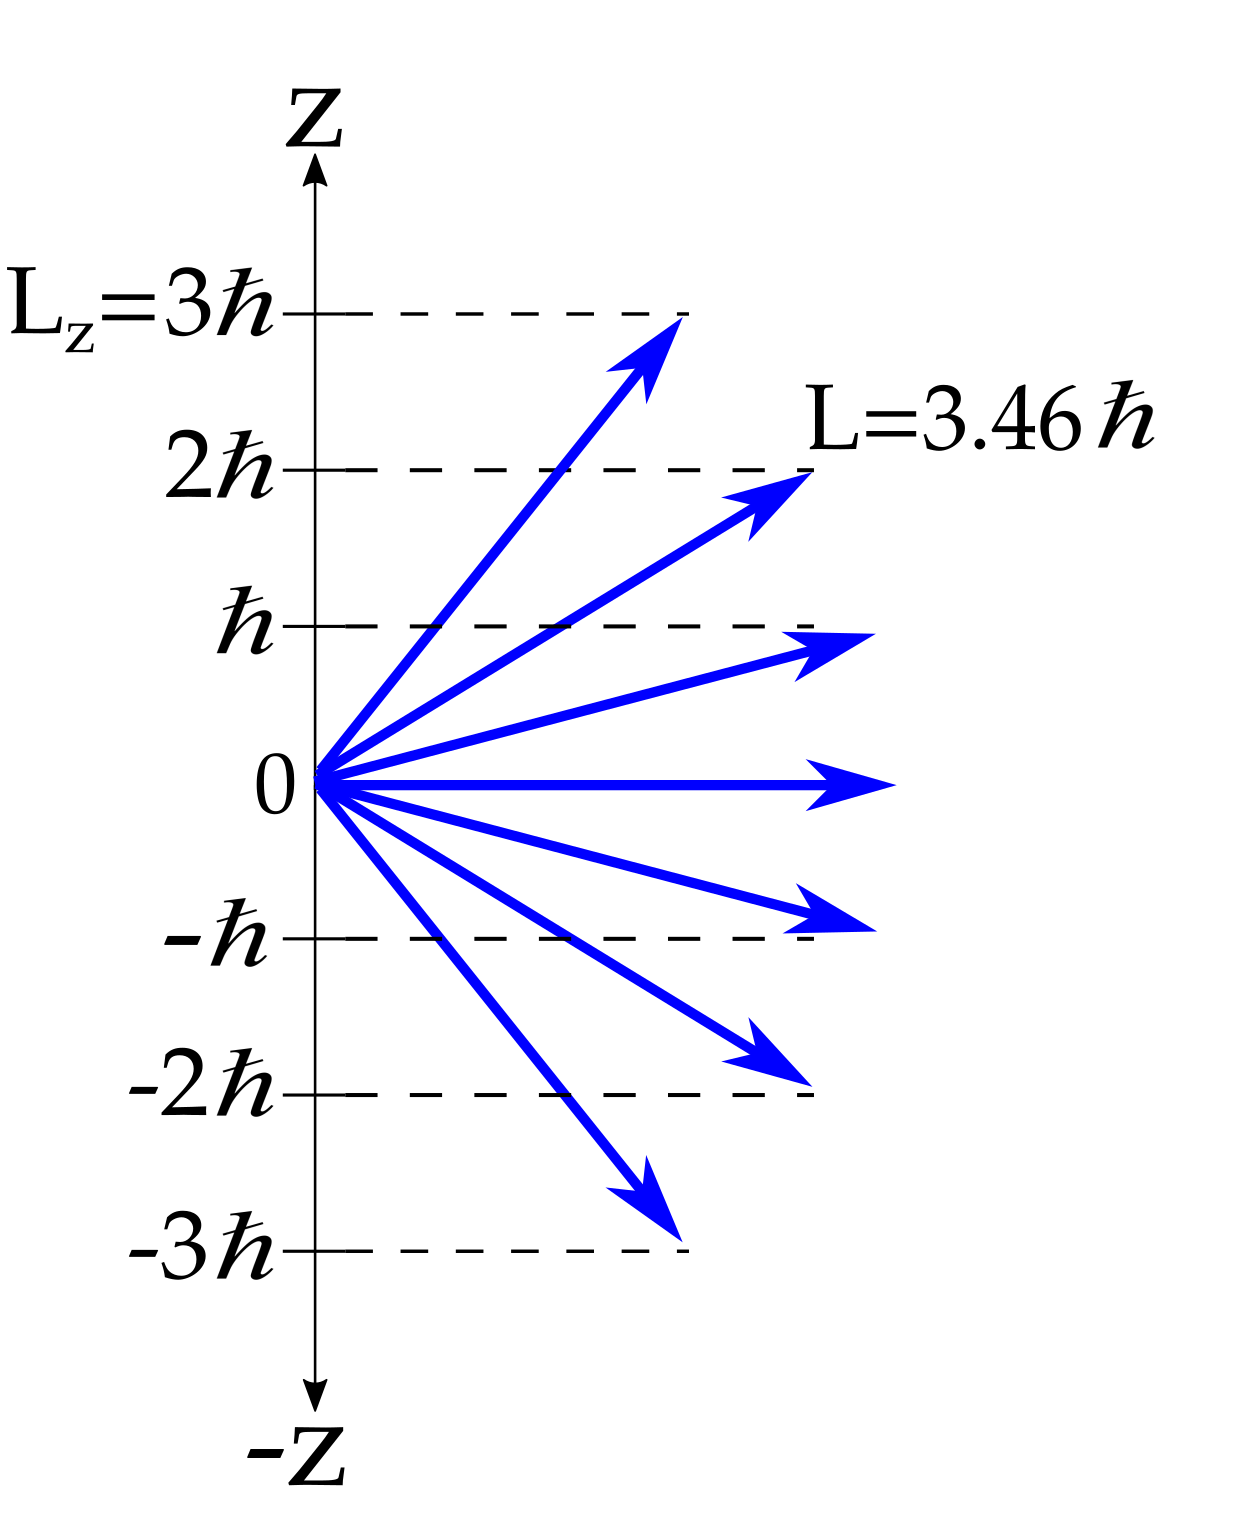
\includegraphics[width=0.6\linewidth]{figs/8.25.png}
        \end{center}
        \item There are $2l+1=7$ orientations.
        \item The magnitude is $L=\sqrt{l(l+1)}\hbar = 3.464\hbar$ so the minimum angle is 
        \begin{equation}
            \theta = \arccos\frac{3}{3.464} = 30^\circ
        \end{equation}
    \end{enumerate}
    \setcounter{enumi}{26}
    \item They differ a lot when $l$ is small, but when $l$ is large, the ratio gets smaller. Note that $\sqrt{l(l+1)}\approx \sqrt{l^2} = l$ for large enough $l$. This should be no surprise, as this is the \emf{correspondence principle.}
    \setcounter{enumi}{36}
    \item For the 1s state of a hydrogen atom, it is
    \begin{equation}
        P(r) = \frac{4}{a_B^3}r^2e^{-2r/a_B},
    \end{equation}
    so 
    \begin{equation}
        \left\langle \frac{1}{r}\right\rangle = \int_0^\infty \frac{1}{r}P(r) \dd{r} = \frac{4}{a_B^3} \int_0^\infty re^{-2r/a_B} = \frac{1}{a_B}
    \end{equation}
    \setcounter{enumi}{40}
    \item This is a calculus answer, which I refuse to do when I can just look up on a table.
    \item Similar to 8.37, we have
    \begin{equation}
        \langle r\rangle = \frac{4}{a_B^3}\int_0^\infty r e^{-2r/a_B} = \frac{3a_B}{2} ,
    \end{equation}
    where I have spared the messy details of integration.

    \emf{Remarks:} Note that $\langle r\rangle \neq \left\langle \frac{1}{r}\right\rangle^{-1}$. Can you figure out (intuitively) why $\langle r\rangle$ is bigger?
    \item Again, this is messy integration. We have
    \begin{equation}
        \frac{4}{a_B^3}\int_{a_B}^{\infty} r^2e^{-2r/a_B} \dd{r} = 5e^{-2} \approx 0.678.
    \end{equation}
    \emf{Remarks:} This doesn't depend on $a_B$, which is expected. Can you justify this via a dimensional analysis?
    \setcounter{enumi}{46}
    \item \begin{enumerate}
        \item The angular Schrodinger equation is 
        \begin{equation}
            \frac{1}{\sin\theta}\frac{d}{d\theta}\left(\sin\theta\frac{d\Theta}{d\theta}\right) + \left(l(l+1)-\frac{m^2}{\sin^2\theta}\right)\Theta = 0.
        \end{equation}
        Plugging in $l=1$ and $m= \pm 1$, then substituting in $\Theta(\theta)=\sin\theta$, we get
        \begin{align*}
            \frac{1}{\sin\theta}\frac{d}{d\theta} \left(\sin\theta \cos\theta\right) + \left(2-\frac{1}{\sin^2\theta}\right)\sin\theta &= \frac{\cos2\theta}{\sin\theta} + 2\sin\theta - \frac{1}{\sin\theta}
        \end{align*}
        Using some trig identities (namely $\cos2\theta = 1-2\sin^2\theta$,) we can show that this indeed reduces to zero, and thus the complete wavefunction is as desired.
    \item We have
    \begin{align}
        \psi_{2,1,1} + \psi_{2,1,-1} &= R_{2p}(r)\sin\theta\left(e^{i\phi}+e^{-i\phi}\right) \\
        &= 2R_{2p}(r)\sin\theta\cos\phi
    \end{align}
    We can use the relationship $R_{2p}(r) = Are^{-ir/2a_B}.$ Noting that $x=r\sin\theta\cos\phi$ in spherical coordinates, the sum becomes $2Axe^{-r/2a_B} = 2\phi_{p_x}.$ Similarly, when we take the difference, and using $e^{i\phi}-e^{-i\phi} = 2\sin\phi$, we end up with 
    \begin{equation}
        \phi_{2,1,1}-\phi_{2,1,-1} = 2iAye^{-r/2a_B} = 2i\phi_{p_y}.
    \end{equation}
    \end{enumerate}
    \setcounter{enumi}{48}
    \item Equation (8.108) gives us
    \begin{equation}
        R(r) = Ar^{n-1}e^{-r/na_B}
    \end{equation}
    for $l=n-1$. The radial probability density is 
    \begin{equation}
        P(r) = 4\pi r^2 R(r)^2 = 4\pi A^2 r^{2n}e^{-2r/na_B}
    \end{equation}
    To find the most probable radius, we find when $P'(r)=0.$ Doing so then $r=n^2a_B.$

    \emf{Remarks:} I'm pretty sure equation 8.108 is wrong lol. It's missing a factor of $n$ (which I have included in my answer.)
    \item Recall that we have 
    \begin{align*}
        P_{2s}(r) = 4\pi A^2 r^2 \left(2-\frac{r}{a_B}\right)^2 e^{-r/a_B} \\ 
        P_{2p}(r) = 4\pi A^2 r^4 e^{-r/a_B}
    \end{align*}
    We end up with $r=5.24a_B$ and $r=0.76a_B$ for the 2s and 2p states, respectively. Note that for the $2s$ case, there will be two extremes. We need to compare the values at each to determine which is the most probable.
    \item For $\text{Ni}^{27+}$, the effective atomic number is $Z=27$, so we have $a = \frac{a_B}{27}$ for the most probable electron radius. Since its hydrogen-like, the ground state energy is 
    \begin{equation}
        E = -27^2 \frac{E_R}{1^2} = -729E_r,
    \end{equation}
    and the binding energy is the negative of this.
\end{enumerate}
\end{document}